\documentclass[a4paper,14pt]{article}

\usepackage{comment} % Para comentar várias linhas ao mesmo tempo

%matemática
\usepackage{amsmath}
\usepackage{amssymb}

%diagramação
\usepackage{extsizes}
\everymath{\displaystyle}
\usepackage{geometry}
\usepackage{fancyhdr}
\usepackage{multicol}
\usepackage{graphicx}
\usepackage[brazil]{babel}
\usepackage[shortlabels]{enumitem}
\usepackage{cancel}
\usepackage{textcomp}
\usepackage{tcolorbox}

%tabelas
\usepackage{array} % Para melhor formatação de tabelas
\usepackage{longtable}
\usepackage{booktabs}  % Para linhas horizontais mais bonitas
\usepackage{float}   % Para usar o modificador [H]
\usepackage{caption} % Para usar legendas em tabelas
\usepackage{wrapfig} % Para usar tabelas e figuras flutuantes
\usepackage{xcolor} % Para cores do fundo de tabelas
\usepackage{colortbl} % Para cores do fundo de tabelas

%tikzpicture
\begin{comment}
	\usepackage{tikz}
	\usepackage{scalerel}
	\usepackage{pict2e}
	\usepackage{tkz-euclide}
	\usetikzlibrary{calc}
	\usetikzlibrary{patterns,arrows.meta}
	\usetikzlibrary{shadows}
	\usetikzlibrary{external}
\end{comment}


%pgfplots
\usepackage{pgfplots}
\pgfplotsset{compat=newest}
\usepgfplotslibrary{statistics}
\usepgfplotslibrary{fillbetween}

%colours
\usepackage{xcolor}



\columnsep=2cm
\hoffset=0cm
\textwidth=8cm
\setlength{\columnseprule}{.1pt}
\setlength{\columnsep}{2cm}
\renewcommand{\headrulewidth}{0pt}
\geometry{top=1in, bottom=1in, left=0.7in, right=0.5in}

\pagestyle{fancy}
\fancyhf{}
\fancyfoot[C]{\thepage}

\begin{document}
	
	\noindent\textbf{6FMA88 - Matemática} 
	
	\begin{center}Polígonos: introdução (Versão estudante)
	\end{center}
	
	\noindent\textbf{Nome:} \underline{\hspace{10cm}}
	\noindent\textbf{Data:} \underline{\hspace{4cm}}
	
	%\section*{Questões de Matemática}
	
	\begin{multicols}{2}
		\noindent \begin{itemize}
			\item Polígonos são figuras planas fechadas resultantes da união de segmentos de reta. Os segmentos denominam-se lados e as extremidades dos segmentos são os vértices do polígono. De acordo com o número de lados, cada polígono recebe um nome. Exemplos: o hexagono tem 6 lados, o decágono tem 10 lados e o $n$-ágono tem $n$ lados.
			\item Sendo $\gamma$ o conjunto formado por um polígono qualquer e seu interior, o polígono é chamado de convexo se, e somente se, $\forall$A, $B \subset \gamma$, $\overline{AB} \subset \gamma$.
		\end{itemize}
		\noindent\textsubscript{-----------------------------------------------------------------------}
		\begin{enumerate} 
			\item Nos itens a seguir, dizer quais são polígonos convexos e quais são polígonos não convexos.
			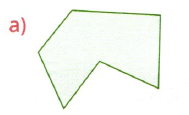
\includegraphics[width=1\linewidth]{6FMA88_imagens/imagem1}
			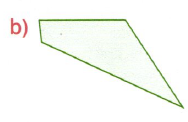
\includegraphics[width=1\linewidth]{6FMA88_imagens/imagem2}
			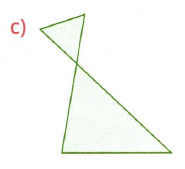
\includegraphics[width=1\linewidth]{6FMA88_imagens/imagem3}
			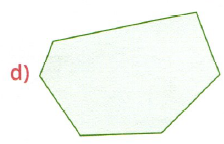
\includegraphics[width=1\linewidth]{6FMA88_imagens/imagem4}
			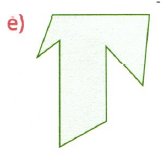
\includegraphics[width=1\linewidth]{6FMA88_imagens/imagem5}
			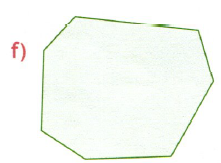
\includegraphics[width=1\linewidth]{6FMA88_imagens/imagem6}
			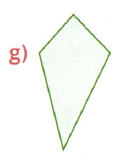
\includegraphics[width=1\linewidth]{6FMA88_imagens/imagem7}
			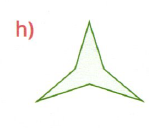
\includegraphics[width=1\linewidth]{6FMA88_imagens/imagem8}
			\item Com base no número de lados, qual o nome que cada polígono convexo do exercício anterior recebe? \\\\\\\\\\\\\\
			\item Quantos vértices têm os polígonos convexos de:
			\begin{enumerate}[a)]
				\item 4 lados? \\\\\\\\
				\item 24 lados? \\\\\\\\
				\item 13 lados? \\\\\\\\
				\item 59 lados? \\\\\\\\
				\item 100 lados? \\\\\\\\
				\item $n$ lados? \\\\\\\\
			\end{enumerate}
			\item Quantos lados tem:
			\begin{enumerate}[a)]
				\item o heptágono? \\\\\\\\
				\item o undecágono? \\\\\\\\
				\item o pentadecágono? \\\\\\\\
				\item o hexágono? \\\\\\\\\\\\
				\item um polígono convexo de 21 vértices? \\\\\\\\
				\item um polígono de 53 vértices? \\\\\\\\
			\end{enumerate}
			\item Usando a malha pontilhada abaixo e uma régua, una os pontos formando um triângulo, um pentágono e um octógono. \\\\
			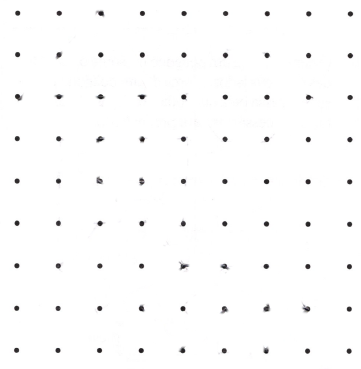
\includegraphics[width=1\linewidth]{6FMA88_imagens/imagem9}
			%57 a 60
			\item Quantos lados tem o:
			\begin{enumerate}[a)]
				\item pentadecágono? \\\\\\
				\item icoságono? \\\\\\
				\item decágono? \\\\\\
				\item octógono? \\\\\\
				\item dodecágono? \\\\\\
				\item $n$-ágono? \\\\\\
			\end{enumerate}
			\item Quantos vértices tem o:
			\begin{enumerate}[a)]
				\item quadrilátero? \\\\\\
				\item triângulo? \\\\\\
				\item heptágono? \\\\\\
				\item polígono convexo de 16 lados? \\\\\\
				\item polígono convexo de 35 lados? \\\\\\
				\item polígono convexo de 60 lados? \\\\\\
			\end{enumerate}
			\item Quantos lados tem:
			\begin{enumerate}[a)]
				\item um pentágono? \\\\\\
				\item um eneágono? \\\\\\
				\item um hexágono? \\\\\\
				\item um polígono convexo de 17 vértices? \\\\\\
				\item um polígono convexo de 28 vértices? \\\\\\
				\item um polígono convexo de 41 vértices?
			\end{enumerate}
			\item Um undecágono é um polígono que tem:
			\begin{enumerate}[a)]
				\item 6 lados
				\item 8 lados
				\item 11 lados
				\item 15 lados
				\item 21 lados
			\end{enumerate}
		\end{enumerate}
	\end{multicols}
\end{document}